\documentclass{article}
\usepackage{packages}

\title{\textbf{Fundamentals of Simulation Methods} \\ \vspace{5pt} \large University of Heidelberg, WiSe 2021/2022 \\ \vspace{5pt} Mandatory assignements - Set 1}
\date{\textbf{Date:} \today}
\author{\textbf{Author:} Matteo Zortea}

\begin{document}
\maketitle

\section*{Exercise 1}
    Let us denote the basis in which we are representing the numbers by a subscript. For example $(3)_{10}$ means that 3 is written in the decimal basis. \\
    Let us first consider number of the type $(1.X)_{10}$. In the binary basis these numbers are of the type $(1.Y)_2$, i.e. only one bit is used for the integer part, which is always 1. \\
    In the IEEE-754 standard representation one has 23 bits available for the mantissa when using single precision and 51 when using double precision. \\
    Since the exponent in this representation for these numbers is fixed, one has that all the possible combination of numbers within $1$ and $2$ are $2^{23}$ for the single precision case
    and $2^{51}$ for the double precision case. \par
    \vspace{15pt}
    On the other side numbers of the type $(255.X)_{10}$ have a binary representation of the type $(11111111.Y)_2$, which becomes 
    $(1.1111111Y \times 2^Z)_2$ when written in the IEEE-754 format. The operation of shifting the point put contraints on the first 7 digits of the mantissa, that is all the numbers of the type $(255.X)_10$ have the same first 7 digits in the mantissa when represented in the IEEE-754 standard.
    Since the number of digits available to represent the mantissa does not change we are now left with only $23-7=16$ usable digits for the single precision and $51-7=44$ for the double precision. This means that in the given interval we can represent only $2^{16}$ numbers in the single precisoin format 
    and $2^{44}$ in the double precision format.

\section*{Exercise 2}
\subsubsection*{1)}
This is an automatic cast problem. In the case of $y$, when performing the division $i/2$, we are dividing two integers. By convention the type of the result is considered int itself, so that the decimal part is truncated. \\\
When the result of the multiplication by 2 is stored into $y$ the result is casted to double, but the decimal part was lost before. \\
In the case of $z$, when performing the division $i/2.$ we are dividing a integer by a floating point number, and this conventionally is stored in a floating point variable. When storing the result of the multiplication by 2 
the number is casted to double, which increase the precision for successive operation but has no influence of what happened before i.e. at that point the number still have single precision.
\subsubsection*{2)}
The correct one is $x$. In the case of $y$, when performing $b+c$, we are small summing a number ($c$) to very big number ($b$) and in particular the value of $c$ is so small compared to $b$ that the result of the sum is still $b$, i.e. we don't have enough resolution to store the variation caused by $c$.
\subsubsection*{3)}
The number $x*x$ exceeds the maximum representable number in the floating point format which is $2^{128} \simeq 3.4 \times 10^{38}$. Hence an overflow happens and the number is stored as $+inf$.

\newpage 

\section*{Exercise 3}
\begin{figure}[h]
    \centering 
    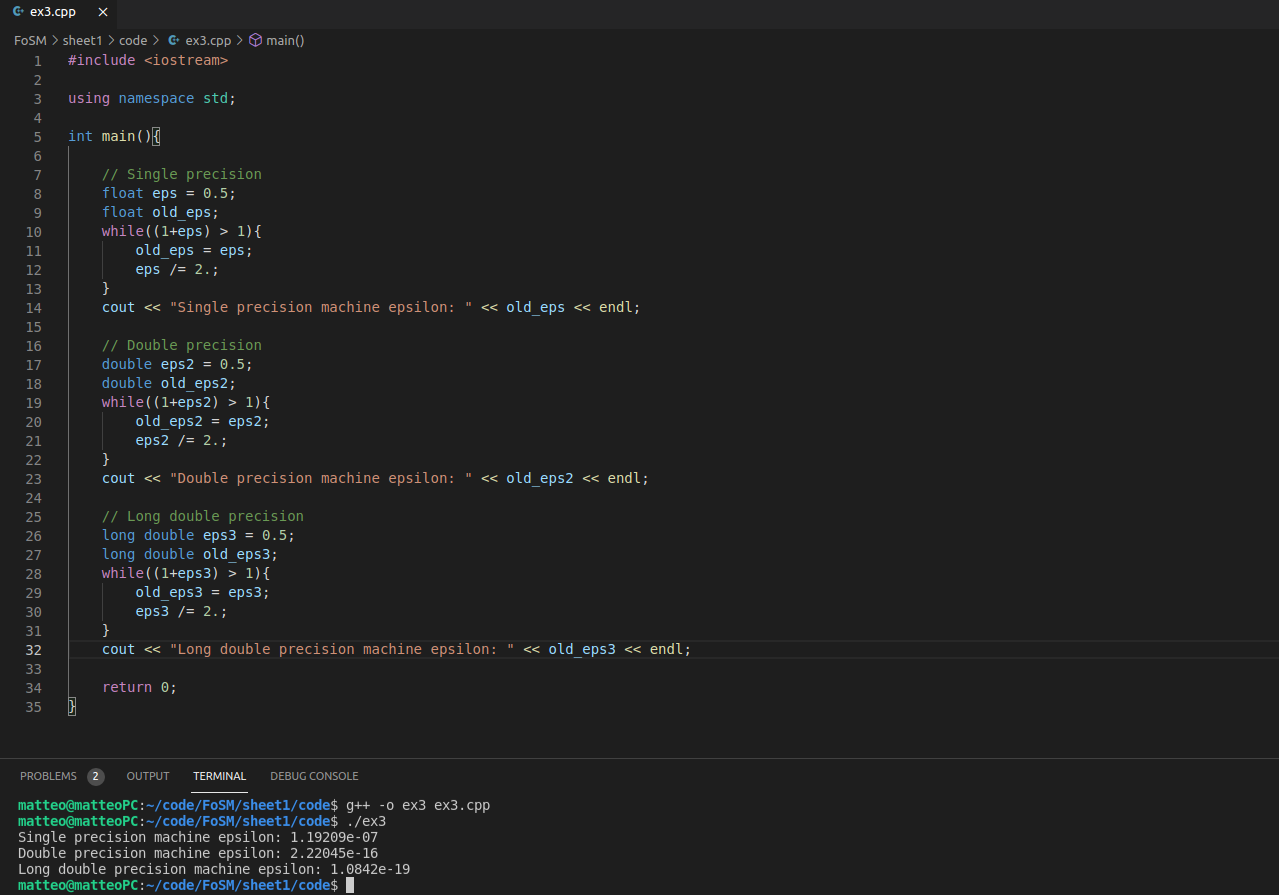
\includegraphics[scale=0.35]{pics/machine_eps.png}
    \caption{Program that evaluates machine $\epsilon$ for single, double and long double precision}
    \label{fig:machine_epsilon}
\end{figure}
When we try to print $1+\epsilon$ the terminal shows just $1$. Thus, if we increase the number of digits printed (e.g. by using setprecision(n) in c++) we can see that after some digits, some are non-zero.

\section*{Exercise 4}
\subsubsection*{1)}
\begin{equation*}
    f(x)=\frac{x+\exp (-x)-1}{x^{2}} = \frac{x + \left(1 - x + \frac{x^2}{2} + o(x^2)\right) - 1}{x^2} = \frac{\frac{x^2}{2} + o(x^2)}{x^2} \qquad \Longrightarrow \qquad \lim_{x \to 0} f(x) = \frac{1}{2}
\end{equation*}
\subsubsection*{2)}
Please see attached code.
\subsubsection*{3)}
Please read outputdata.csv to see the output of the program. \\
For $x > 10^{-5}$ there is a clear growing pattern in the results (approaching $0.5$ from below), and the evaluation can be considered reliable up to the fifth decimal digit. Then the fifth digit start oscillating significantly and the the
evaluation method proposed in point 5 is more reliable. \\
For $10^{-8} < x < 10^{-7}$  the function starts deviating significantly to the expected value, and the result is no more reliable. \\
Fof $x < \times 10^{-8}$ the result is completely wrong, and it yields $0$ instead of $0.5$.
\subsubsection*{4)}
For small $x$ the number $\exp(-x)$ is close to $1$, so close that one must go through many decimal digits before getting one different from 9. This means that, due to finite byte representation, 
as $x$ gets smaller we have one point in which the decimals that differ from $9$ in the exponential are not stored anymore and get truncated. When we then sum $x$ to this number, all the most significant digits are 0 since the sum should be a number 
of the type $1.000\dots x$ with $x$ beeing the first decimal number that differs from 0. The fact is that this number is truncated sign this digit was not significant before the sum.
\subsubsection*{5)}
If $x$ is less than $1e-5$ we can use a taylor expansion around $x=0$ for the exponential, which yields the expression
\begin{equation*}
    f(x) = \frac{1}{2} + \frac{x}{6} + \frac{x^2}{24} + o(x^2)
\end{equation*}
In the program I kept the first 30 terms of the series (please see attached code) and it yields the correct result.
\end{document}